\documentclass[12pt]{article}
\usepackage[margin=1.5cm]{geometry}
\usepackage{parskip}
\usepackage{amsmath}
\usepackage{amssymb}
\usepackage{amsfonts}
\usepackage{enumitem}
\usepackage{graphicx}
\usepackage{stmaryrd}
\graphicspath{ {./images/} }


\begin{document}
\begin{enumerate}[label=(\alph*)]

  \item
    The Nussinov algorithm for RNA folding is an algorithm designed to predict the most likely folding structure of an RNA sequence.

    The algorithm is a dynamic programming algorithm, and works by considering 4 cases: left mismatch, right mismatch, match, or bifurcation.

    The function looks like:

    $\gamma(i,j) = \max \begin{cases}\gamma(i+1, j)\\\gamma(i, j-1)\\\gamma(i+1, j-1) + \delta(i,j)\\\max_{i < k < j}(\gamma(i,k) + \gamma(k+1, j))\end{cases}$

    Where we initialise with $\gamma(i, i) = 0$ and $\gamma(i, i-1) = 0$, and $\delta(i,j) = 1$ if $x_i$ and $x_j$ are a complementary base pair, and $\delta(i,j) = 0$ otherwise.

    To compute this function for a single $i,j$, it takes $O(|x|)$ time, since the last case (bifurcation) requires searching for the two loops.

    Since we have to fill an $|x| \times  |x|$ grid, the whole algorithm takes time $O(|x|^3)$ (and $O(|x|^2)$ space to hold the grid).

    As a small example, consider the string \texttt{AGCU}

    We get:

    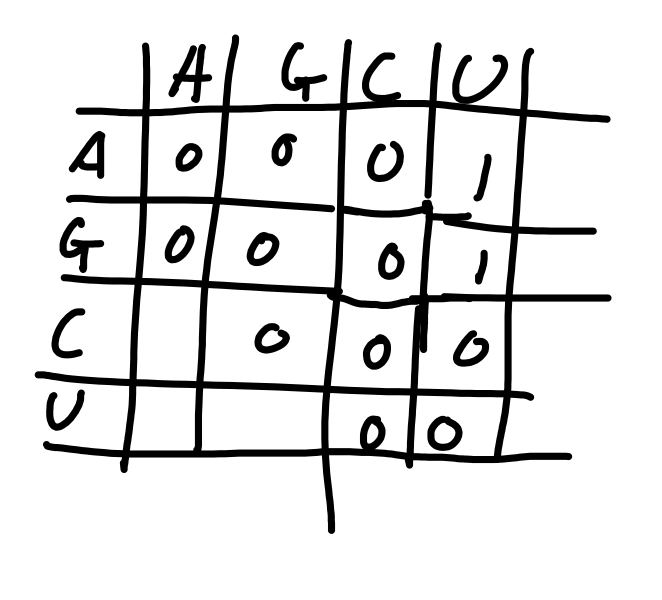
\includegraphics[scale=0.3]{nussinov}

  \item
    Not relevant.

  \item
    \begin{enumerate}[label=(\roman*)]

      \item
        To build such an HMM to identify genes in a genome sequence, we need to design our model. In this case, we might choose the genes to be the hidden states, and the emissions to be the bases, such that the sequence of emissions gives us our genome sequence.

        If we had a transition probability matrix and emission probability matrix, we could then run the Viterbi algorithm on a genome sequence to give us the most likely hidden states, and thus most likely genes, for our genome sequence.

        So, our problem then becomes to find a transition probability matrix and emission probability matrix. If we had a dataset of genome sequences and manually tagged genes, then we could use this to train our HMM to find the transition probability matrices and emission probability matrices.

      \item
        To assess the sensitivity and specificity of an HMM, we need some ground truth data. After using our HMM, we can then count the number of times we correctly predicted a gene, and divide by the number of times we actually knew the underlying gene in our ground truth data. This is the sensitivity, or true positive rate.

        The specificity is then given by the total number of times we predicted a gene correctly divided by the number of times we predicted a gene overall).
        
    \end{enumerate}



        
    \end{enumerate}
\end{document}
